\section{Fluxional execution model} \label{section:model}

Many frameworks for distributed systems are renowned for their performances\cite{Akidau2013, Jain2006, Marz2011, Welsh2000, Wu2007, Zaharia2010}.
However, we focus on a compilation approach to replace the shift in programming model rather than the performance of the runtime.
We present in this section an extremely simplified but generic execution model inspired by the literature, only to support the confirmation of feasibility for the compilation process detailed in section \ref{section:compiler}.
The execution model is not distributed on remote machines, however it isolates the execution of fluxions in different processes to reproduce the execution conditions of a distributed execution model.
We are interested in the problems arising from this isolation.

\subsection{Fluxions and workers}

The fluxional execution model manages and invokes autonomous execution units named fluxion $\bnfpn{flx}$.
A fluxion is composed of a unique name $\bnfpn{id}$, a processing function $\bnfpn{fn}$, and a persisted memory called a \textit{context} $\bnfpn{ctx}$.
Its function $\bnfpn{fn}$ consumes an input stream $\bnfpn{stream}$ and generates one or more outputs streams to other fluxions $\bnfpn{dest}$.
The \textit{context} persists the state on which a fluxion rely between two message receptions.
At a message reception, the fluxion modifies its \textit{context}, and sends back messages to downstream fluxions.
A message is composed of the recipient fluxions' names and a body.

Fluxions are executed on workers.
A worker is an event-loop and an isolated heap ; it is a \textit{Node.js} instance.
The context of a fluxion is lexically isolated.
It has a distinct lexical scope containing variables not shared with any other fluxion.
However, fluxions on the same worker share the same event-loop, and the same heap ; they can send references to each over.
Fluxions on different workers have different event-loops and heaps ; their communications are serialized, so it impossible to send heap references.
Fluxions are the stages in a pipeline architecture.
The streams of messages between fluxions are carried by the messaging system.

The event-loop assures the exclusivity and atomicity of operations of each fluxion on the heap.
\comment{The following sentence is poorly constructed}
This organization shows that the more the memory is shared, the harder it is to distribute fluxions on different workers to allow parallelisation of their execution.

\begin{bnf*}
  \bnfprod{program}    {\bnfpn{flx} \bnfor \bnfpn{flx} \bnfsp \bnftd{eol} \bnfsp \bnfpn{program}}\\
  \bnfprod{flx}        {\bnfts{\texttt{flx}} \bnfsp \bnfpn{id} \bnfsp \bnfpn{ctx} \bnfsp \bnfpn{worker} \bnfsp \bnftd{eol} \bnfsp \bnfpn{streams} \bnfsp \bnftd{eol} \bnfsp \bnfpn{fn}}\\
  \bnfprod{worker}     {\bnfts{\texttt{on}} \bnfsp \bnfpn{id} \bnfor \bnftd{empty string}}\\
  \bnfprod{streams}    {\bnfts{\texttt{null}} \bnfor \bnfpn{stream} \bnfor \bnfpn{stream} \bnfsp \bnftd{eol} \bnfsp \bnfpn{streams}}\\
  \bnfprod{stream}     {\bnfpn{op} \bnfsp \bnfpn{dest} \bnfsp [\bnfpn{msg}]}\\
  \bnfprod{dest}       {\bnfpn{list}}\\
  \bnfprod{ctx}        {\bnfts{\texttt{\{}} \bnfpn{list} \bnfts{\texttt{\}}}}\\
  \bnfprod{msg}        {\bnfts{\texttt{[}} \bnfpn{list} \bnfts{\texttt{]}}}\\
  \bnfprod{list}       {\bnfpn{id} \bnfor \bnfpn{id} \bnfsp \bnfts{,} \bnfsp \bnfpn{list}}\\
  \bnfprod{op}         {\bnfts{\texttt{>}\texttt{>}} \bnfor \bnfts{\texttt{-}\texttt{>}}}\\
  \bnfprod{id}         {\bnftd{Javascript identifier}}\\
  \bnfprod{fn}         {\bnftd{Javascript and stream syntax}}\\
\end{bnf*}
\vspace{-1.5\baselineskip}~\\

We represent here the syntax of a high-level language to represent a program in the fluxionnal form.
It is the target for our compiler.

\subsection{Messaging system}

In a distributed approach, the messages between fluxions would be carried over a distributed message broker.
However this execution model is only a simulation of a distributed execution environement.
We simplify the distributed message broker with a master message queue, but each worker still has its own message queue.
% The messaging system is the core of the execution model.
% It carries messages and invokes fluxions at reception.

The messaging system sends messages to the isolated worker hosting the destination fluxion.
The worker containing the messaging system locally hosts fluxions that need access to the external network.
% Using a message queue allows to execute multiple processing chains fairly and concurrently, without difference in scheduling local messages, or network messages.
The life cycle of a fluxional application is illustrated in figure \ref{fig:MesSys}.

\begin{figure}[h!]
  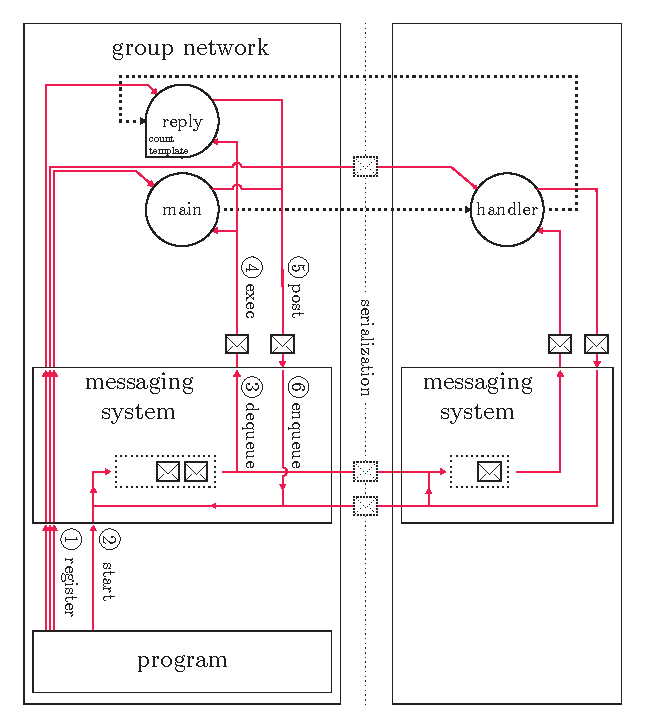
\includegraphics[width=\linewidth]{ressources/schema-message.pdf}
  \caption{Messaging system details}
  \label{fig:MesSys}
\end{figure}

The messaging system carries messages based on the names of the recipient fluxions.
If two fluxions share the same name, it would lead to a conflicting situation for the messaging system.
Every fluxion needs to be registered with a unique name.
This registration associates a processing function with a unique name and an initial \textit{context}.
The registration is done using the function \texttt{register(<name>, <fn>, <context>)}, \circled{1}.
% A fluxion can dynamically register other fluxions

To trigger a chain of fluxions, a message is sent using the function \texttt{start(<msg>)}, \circled{2}.
This first message represent the incoming of a request from a user.
% This function pushes a first message in the queue.
The system dequeues this message and dispatch it to the destination fluxion, \circled{3} and \circled{4}.
The recipient function sends back messages from the isolated worker using the function \texttt{post(<msg>)}, \circled{5}, to be enqueued in the centralised message queue, \circled{6}.
The system loops through steps \circled{3} and \circled{4} until the queue is empty.
This cycle starts again for each new incoming request causing a \textit{start} message.

Algorithms \ref{alg:parcours} and \ref{alg:traitement} describe the behavior of the messaging system after the \texttt{start} function invocation.

\begin{algorithm}
\caption{Message queue walking algorithm}
\label{alg:parcours}
\begin{algorithmic}
\Function{loopMessage}{\null}
\While{$msg$ \textbf{presents in} $msgQueue$}
\State $msg \gets$ \Call{dequeue}{\null} \Comment{\circled{3}}
\State \Call{ProcessMsg}{$msg$}
\EndWhile
\EndFunction
\end{algorithmic}
\end{algorithm}

\begin{algorithm}
\caption{Message processing algorithm}
\label{alg:traitement}
\begin{algorithmic}
\Function{processMsg}{$msg$}
\For{$dest$ \textbf{in} $msg.dest$}
\State $worker \gets lookup(dest)$
\State \Call{worker.send}{$fluxion, msg.body$} \Comment{\circled{4}}
% \State $message \gets$ \Call{exec}{$fluxion, msg.body$} \Comment{\circled{4} \& \circled{5}}
% \State \Call{enqueue}{$message$} \Comment{\circled{6}}
\EndFor
\EndFunction
\end{algorithmic}
\end{algorithm}

\subsection{Service example}

To illustrate the fluxional execution model, and the compiler we present an example of a simple web application.
This application reads the file containing its own source code, and sends it back along with a request counter.

The original source code of this application is available on github\cite{flx-example}, and in listing \ref{lst:source}.
In this source code, some points are worth noticing.

\begin{itemize}
  \item The \texttt{handler} function, line 5 to 11, contains the logic we want to split into the fluxional processing chain.
  It receives the user request in the variable \texttt{res} which is used by the last function of the chain, \texttt{reply}.
  \item The \texttt{count} object at line 3 is a persistent memory that increments the request counter.
  This object needs to be mapped to a fluxion \textit{execution context} in the fluxional execution model.
  \item The \texttt{app.get} and \texttt{app.send} methods, respectively line 5 and 9, interface the application with the clients.
  The processing chain of functions occurs between these two functions : $\texttt{get} \twoheadrightarrow \texttt{handler} \to \texttt{readFile} \to \texttt{reply} \to \texttt{send}$.
\end{itemize}

\includecode{js,
  caption={Simple web application. \textnormal{this application replies to every user request with its own source code and the value of a request counter}},
  label={lst:source}
}
{../../flx-example/source.js}

This application is transformed manually into the fluxions chain depicted in Figure \ref{fig:MesSys}. \comment{TODO change the figure to reflect the source, and modify the paragraph below}
We expect a similar result with the compiler described in section \ref{section:compiler}.
Circles represent registered fluxions.
Envelope symbols represent message streams between fluxions with the variables transmitted from one fluxion to the other.
The square in the messaging system holds the \textit{context} of the \texttt{reply} fluxion.
When a new REST request \texttt{GET} is received, a \texttt{start} message triggers the flow.
The \texttt{handler} fluxion receives this \texttt{start} message, reads the source file and forwards it to the \texttt{reply} fluxion which increments the counter, and sends the result back.
Each fluxion propagates the necessary values from one fluxion to the other exclusively by messages.
% Horizontal dashed lines show virtual transmission of messages between fluxions although they all go through the messaging system.

% \begin{figure}[h!]
%   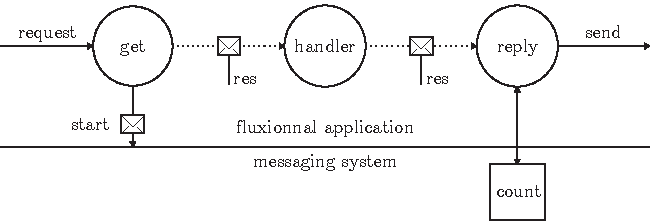
\includegraphics[width=\linewidth]{ressources/flux.pdf}
%   \caption{Fluxions chain manually extracted from the example application}
%   \label{fig:fluxions}
% \end{figure}

\begin{code}[flx, caption={Manual transformation of the example application in our high-level fluxional language},label={lst:fluxional}]
flx get
>> handler [res]
  var app = require('express')(),
      fs = require('fs'),
      count = 0;

  app.get('/', >> handler); @\label{lst:fluxional-streamtohandler}@
  app.listen(8080);
  console.log('>> listening 8080');

flx handler
-> reply [res]
  function handler(req, res) {
    fs.readFile(__filename, -> reply); @\label{lst:fluxional-readfile}@
  }

flx reply {count}
-> null
  function reply(error, data) {
    count += 1; @\label{lst:fluxional-counter}@
    var code = ('' + data).replace(/\n/g, '<br>').replace(/ /g, '&nbsp');
    res.send('downloaded ' + count + ' times<br><br><code>' + code + '</code>' ); @\label{lst:fluxional-ressend}@
  }
\end{code}

The application is organized as follow :
\begin{itemize}
  \item The \texttt{get} fluxion is the \textit{root} fluxion.
  It initializes the application to listen for user requests by calling \texttt{app.get}.
  Every request is forwarded on the stream to the \texttt{handler} fluxion, line \ref{lst:fluxional-streamtohandler}.
  \item The \texttt{handler} fluxion reads the file containing the source code of the application, and forwards the result to the \texttt{reply} fluxion, line \ref{lst:fluxional-readfile}.
  \item The \texttt{reply} fluxion increments the counter, line \ref{lst:fluxional-counter}, formats the reply, and sends it back to the user using the function \texttt{res.send}, line \ref{lst:fluxional-ressend}.
\end{itemize}

\comment{TODO transition missing}
Our goal, as described in the introduction, is not to propose a new programming paradigm with this high-level language but to automate the architecture shift with a compiler.